\section{Relay Channel}

\begin{figure}
    \centering
    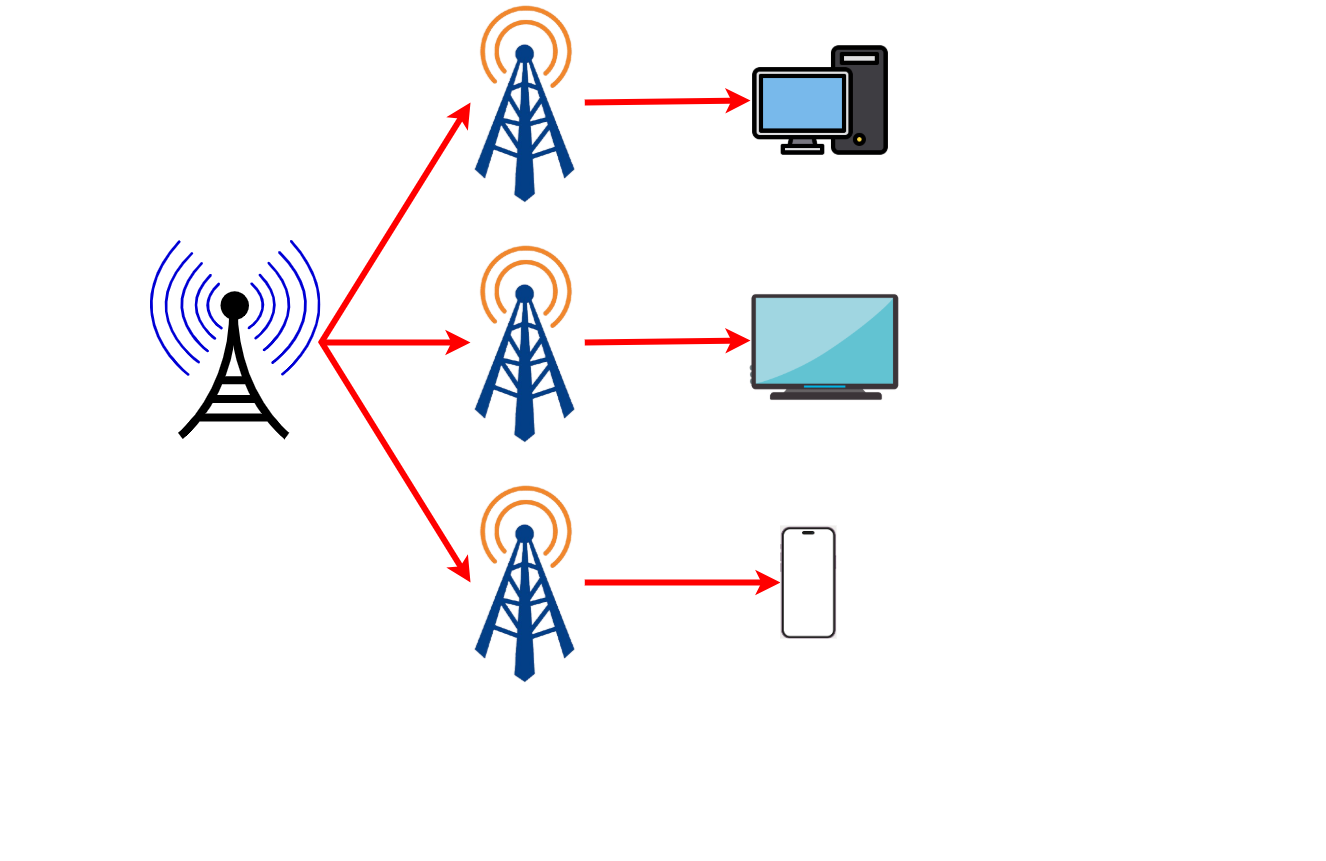
\includegraphics[width=0.5\linewidth]{Presentation Diagrams/RC.png}
    \caption{Enter Caption}
    \label{fig:enter-label}
\end{figure}




%
\begin{tcolorbox}[boxrule=0pt,frame hidden,sharp corners,enhanced, opacityback=0, borderline west={2pt}{0pt}{red}]
\begin{defn} \textbf{(A $(2^{nR},n)$ code} A $(2^{nR}, n)$ code for a relay channel consists of a set of integers $\mathcal{W} = \{1,2,...,2^{nR} \}$, an encoding function
%
\begin{eqnarray}
    X: \{1,2,...,2^{nR}\} \rightarrow \mathcal{X}^n,
\end{eqnarray}
%
a set of relay functions $\{ f_i \}_{i=1}^n$ such that
%
\begin{eqnarray}
    x_{1i} = f_i(Y_{11}, Y_12,...,Y_{1i-1}), \quad 1\leq i \leq n,
\end{eqnarray}
%
and a decoding function,
%
\begin{eqnarray}
    g: \mathcal{Y}^n \rightarrow \{1,2,...,2^{nR}\}.
\end{eqnarray}


\end{defn}
\end{tcolorbox}
%